% !TEX TS-program = xelatex
% !TEX encoding = UTF-8 Unicode
% !Mode:: "TeX:UTF-8"

\documentclass{resume}
\usepackage{zh_CN-Adobefonts_external} % Simplified Chinese Support using external fonts (./fonts/zh_CN-Adobe/)
% \usepackage{NotoSansSC_external}
% \usepackage{NotoSerifCJKsc_external}
% \usepackage{zh_CN-Adobefonts_internal} % Simplified Chinese Support using system fonts
\usepackage{linespacing_fix} % disable extra space before next section
\usepackage{cite}

\usepackage{graphicx}
\usepackage{tabu}
\usepackage{tabularx}
\usepackage{multirow}
\usepackage{progressbar}
\usepackage{setspace}
\usepackage{xpinyin}
\usepackage{float}
\usepackage{booktabs}
\usepackage{wrapfig}
\usepackage{paracol}
\usepackage{etoolbox}
\usepackage{tikz}
\usepackage{fancybox}
\usepackage{psvectorian}
\usepackage{eso-pic}
\usepackage{pgfornament}
\usepackage{fontawesome5}

\definecolor{BodyColor}{HTML}{666666}
\colorlet{body}{BodyColor}
% \definecolor{verdeolivo}{RGB}{85,107,47}
\definecolor{verdeolivo}{RGB}{11, 35, 67}



% 联系方式
\newcommand{\contact}{
    % 根据个人喜好选择字号
    % \small              % 小
    \footnotesize       % 更小
    %\scriptsize         % 再小一号
    \textcolor{white}{
        % 邮箱
        % \faEnvelope \quad \href{mailto:xianhao.y@qq.com}{xianhao.y@qq.com}
        % \hspace{2em}
        % % 手机号
        % \faPhone \quad  (+86)188-220-29021
        % 别的联系方式,如微信、GitHub等
        %  \hspace{2em}
         \faGithub \quad {\sffamily \href{https://github.com/Eilidan}{https://github.com/Eilidan}}
        \hspace{2em}
        \faWechat \quad {\sffamily Eilidan}
        \hspace{2em}
        \faMapMarker \quad {\sffamily 湖北\textperiodcentered 宜昌}
    }
}


\begin{document}
\pagenumbering{gobble} % suppress displaying page number


% % 页眉:校标组合+学院名
% \begin{tikzpicture}[remember picture, overlay]
%   \node[anchor=north, inner sep=0pt](header) at (current page.north){
%       
\includegraphics[width=\paperwidth]{images/header.png}
%   };
%   \node[anchor=west](school_logo) at (header.west){
%       \hspace{0.5cm}
%       
\includegraphics[width=0.35\textwidth]{images/name.png}
%   };
%   \node[anchor=east](school_name) at(header.east){
%       \textcolor{white}{\textbf{机科股份}}
%       \hspace{0.5cm}
%   };
% \end{tikzpicture}




% \begin{tikzpicture}[remember picture, overlay]
%   \node[anchor=south, inner sep=0pt](footer) at (current page.south){
%       
\includegraphics[width=\paperwidth]{images/footer.png}
%   };
%   % 联系方式
%   \node[anchor=center] at(footer.center){\contact};
% \end{tikzpicture}

% \begin{tikzpicture}[remember picture, overlay]
%   \node[opacity=0.05] at(current page.center){
%       
\includegraphics[width=0.9\paperwidth, keepaspectratio]{images/CAMLOGO.png}
%   };
% \end{tikzpicture}


% \AddToShipoutPicture{
%   \begingroup
%   \put(\LenToUnit{2mm},\LenToUnit{\paperheight-2mm}){\pgfornament[anchor=north west,width=2cm]{41}}
% \put(\LenToUnit{\paperwidth-2cm-2mm},\LenToUnit{\paperheight-2mm}){\pgfornament[anchor=north east,width=2cm,symmetry=v]{41}}
% % \put(\LenToUnit{\@tempdimb},\LenToUnit{\@tempdima}){\pgfornament[anchor=south east,width=2cm,symmetry=c]{63}}
% % \put(\LenToUnit{\@tempdima},\LenToUnit{\@tempdima}){\pgfornament[anchor=south west,width=2cm,symmetry=h]{63}}
%   \endgroup
% }

\vspace{0.5cm}
\parbox{2.65cm}{%
\doublebox{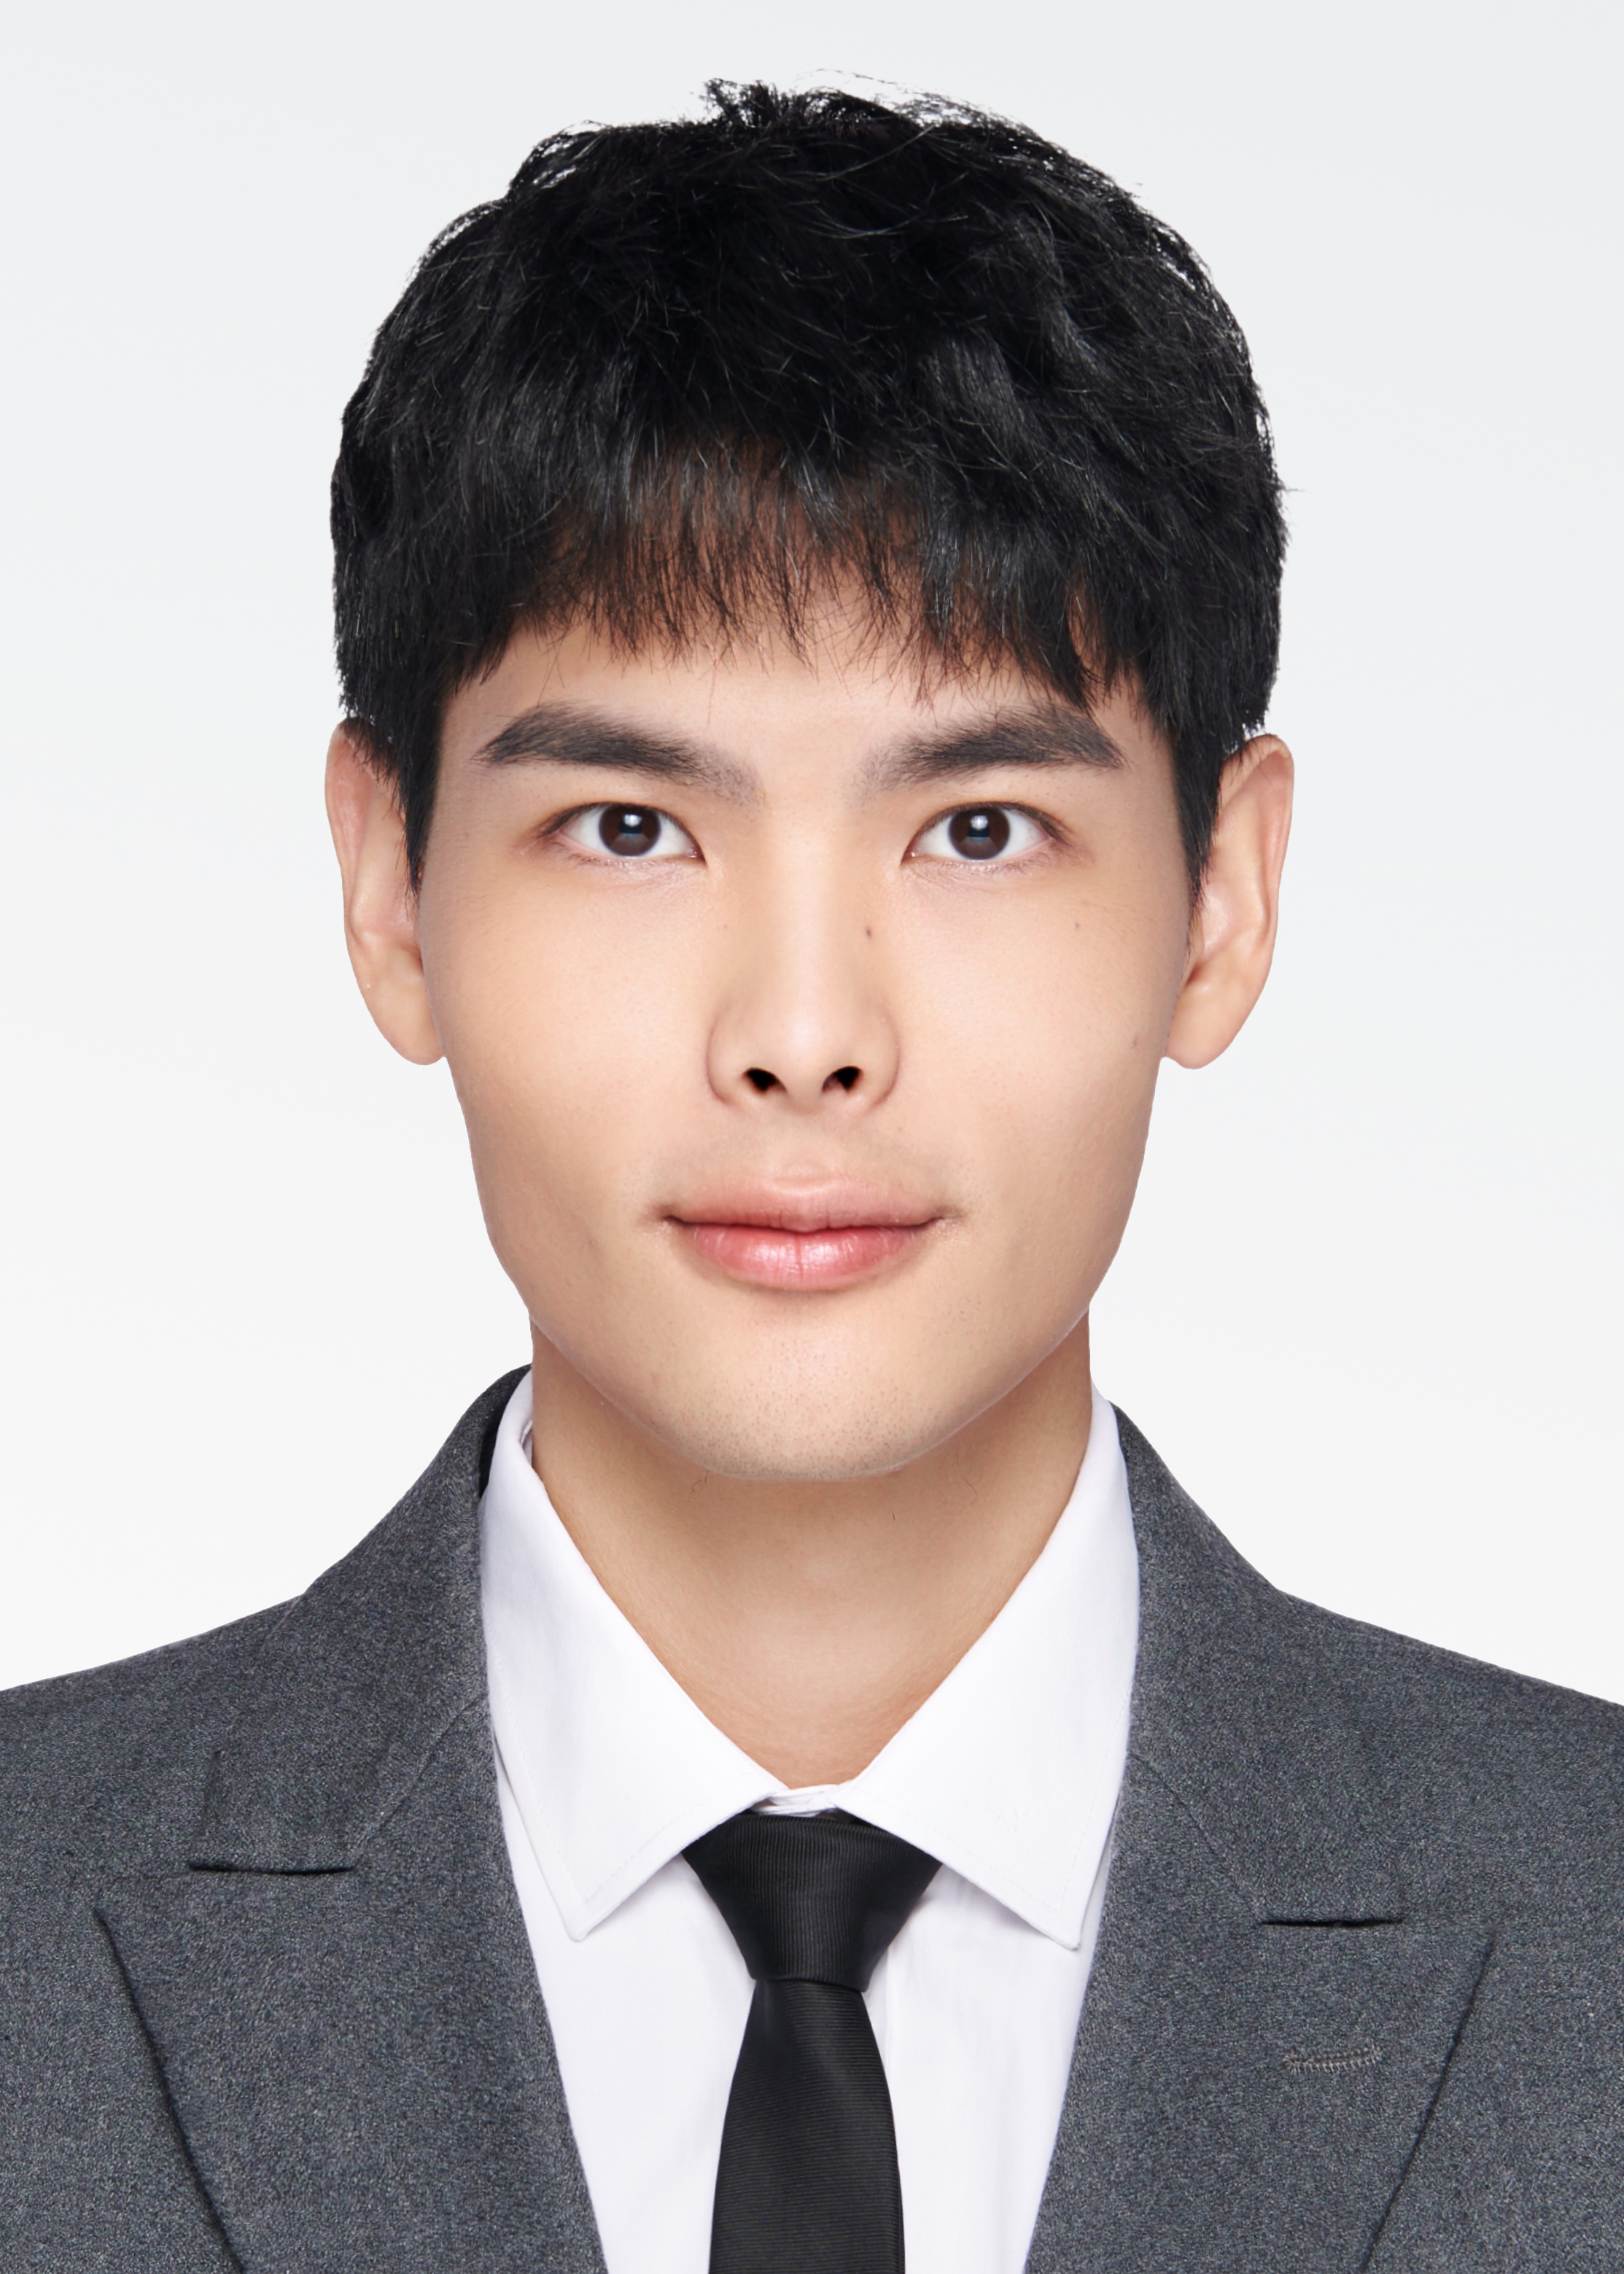
\includegraphics[width=0.88in,clip]{yxh.JPG}}
% \fcolorbox{black}{verdeolivo}{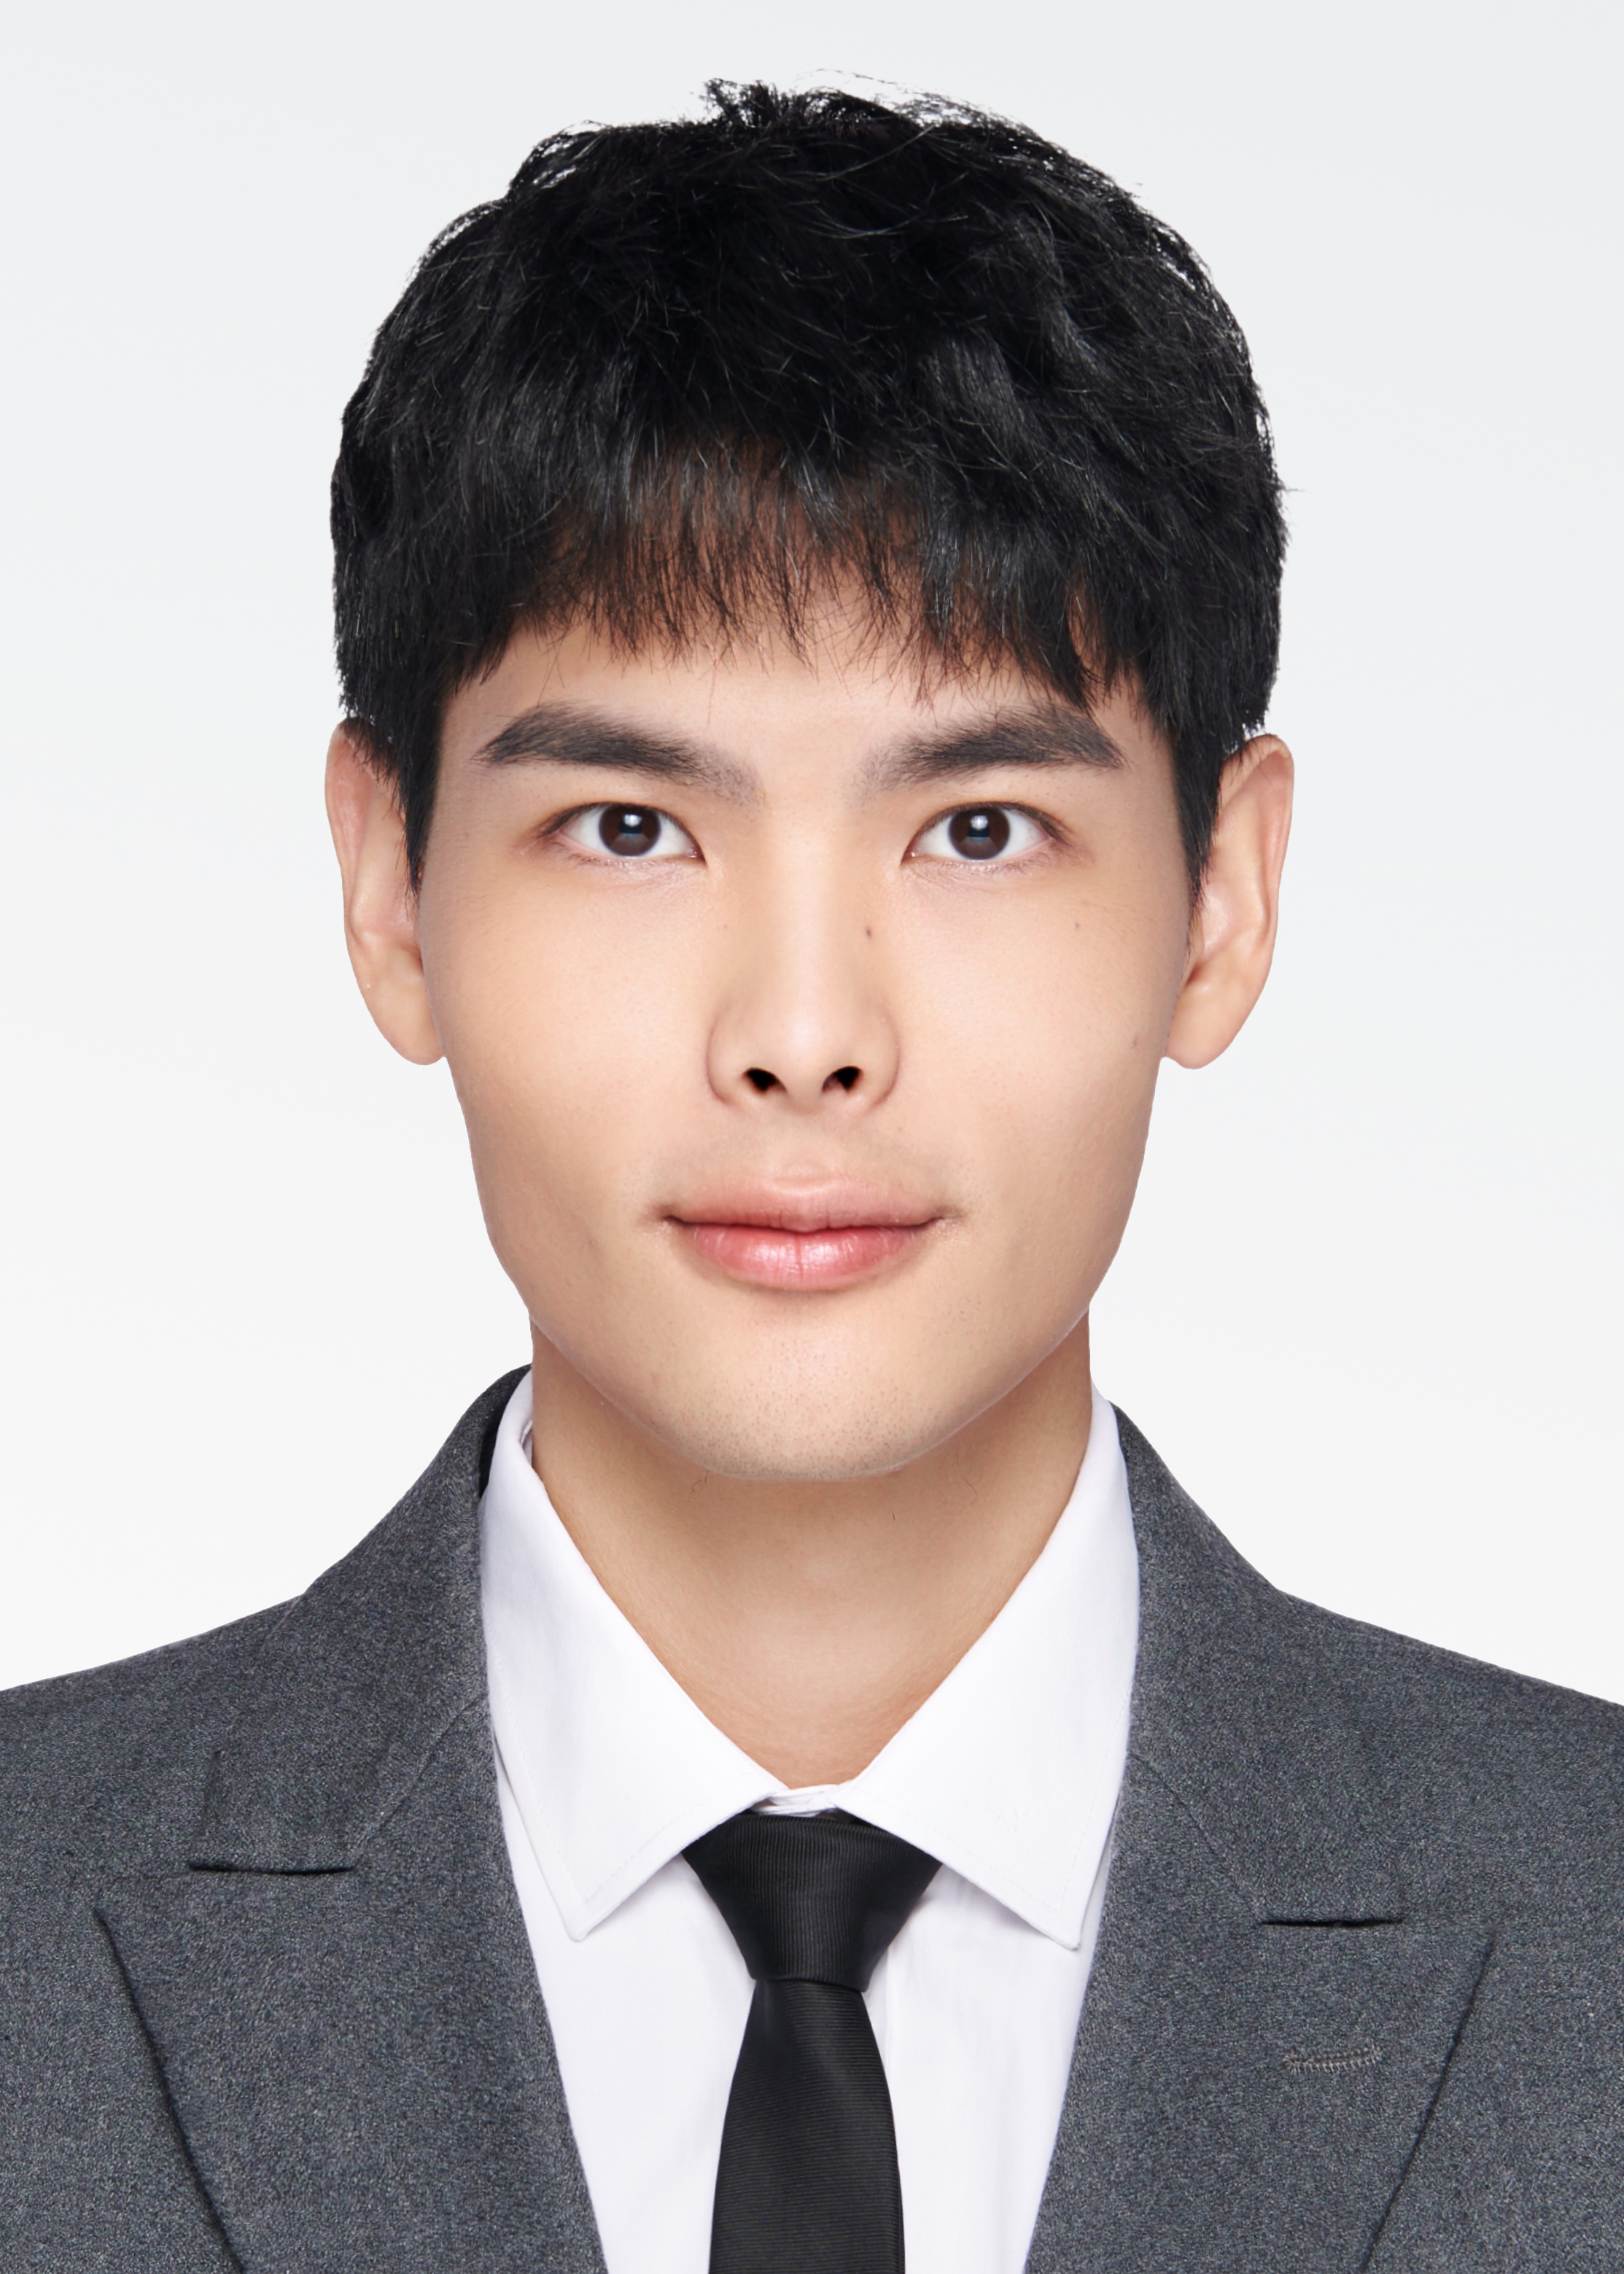
\includegraphics[width=0.88in,clip]{yxh.JPG}}
}
\parbox{0.35cm}{
  \begin{pspicture}(-0.17,-1.5)(0.17,1.5)
    \renewcommand*{\psvectorianDefaultColor}{verdeolivo}
    \rput{90}(0,0){\psvectorian[width=3.5cm]{88}}
  \end{pspicture}
}
% \hspace{0.35cm}
\parbox{7cm}{
  \begin{flushleft}
    \begin{spacing}{1.2}
      
      \email{\scshape{xianhao.y@qq.com}}\\
  \phone{(+86) 188-220-29021}\\
  \institution{中国机械总院\ \textperiodcentered\ 机科股份}\\
  {\color{verdeolivo}\faIcon{github}} \ \href{https://github.com/eilidan/}{\scshape{Eilidan}}\hspace{0.5em}
  {\color{verdeolivo}\faIcon{weixin}} \ \href{https://u.wechat.com/MH5Uz9I93PAiCDcqnYlCZVI?s=2/}{\scshape{Eilidan}}\hspace{0.5em} 
  {\color{verdeolivo}\faIcon{tiktok}} \ \href{https://u.wechat.com/MH5Uz9I93PAiCDcqnYlCZVI?s=2/}{\scshape{Yxllz}}\\
  {\color{verdeolivo}\faIcon{google}} \ \href{yxh741643346200094@gmail.com}{yxh741643346200094@gmail.com}\\
  {\color{verdeolivo}\faIcon{map-marker-alt}} \ 湖北\ \textperiodcentered\ 宜昌\\
    \end{spacing}
  \end{flushleft}
}
\hfill
\parbox{5cm}{
  \begin{pspicture}(-2.6,-2.2)(2.4,2.3)%
    \renewcommand*{\psvectorianDefaultColor}{verdeolivo}%
   %  \psframe[linewidth=0.4pt,fillstyle=solid,fillcolor=white](-8,-5)(8,5)% Ð %haut+bas
    %coins
    % \rput[tl](-3,1.8){\psvectorian[width=1.4cm]{41}}
    % \rput[tr](3,1.8){\psvectorian[width=1.4cm,mirror]{41}}
    % \rput[bl](-3,-1.8){\psvectorian[width=1.4cm,flip]{41}}
    % \rput[br](3,-1.8){\psvectorian[width=1.4cm,flip,mirror]{41}}
    % \psline[linecolor=verdeolivo](-2.88,-0.38)(-2.88,0.38)
    % \psline[linecolor=verdeolivo](2.88,-0.38)(2.88,0.38)
    % \psline[linecolor=verdeolivo](-1.54,-1.743)(1.54,-1.743)
    % \psline[linecolor=verdeolivo](-1.54,1.743)(1.54,1.743)
    \rput(0,0.6){\textbf{\Huge \scshape{杨弦昊}}}
    \rput(0,-0.2){\textbf{\Huge \scshape{XianHao.y}}}
    % \rput[t](0,-0.8){\psvectorian[width=2.6cm]{75}}
    \rput[t](0,-0.7){\psvectorian[width=4cm]{87}}
    % \rput[b](0,1){\psvectorian[width=3.6cm]{45}}
    \end{pspicture}%

  % \begin{pspicture}(-3,-2.2)(3,2.3)%
  %   \renewcommand*{\psvectorianDefaultColor}{verdeolivo}%
  %  %  \psframe[linewidth=0.4pt,fillstyle=solid,fillcolor=white](-8,-5)(8,5)% Ð %haut+bas
  %   %coins
  %   \rput[tl](-3,1.8){\pgfornamenthan[scale=0.2]{14}}
  %   \rput[tr](3,1.8){\pgfornamenthan[scale=0.2,symmetry=v]{14}}
  %   \rput[bl](-3,-1.8){\pgfornamenthan[scale=0.2,symmetry=h]{14}}
  %   \rput[br](3,-1.8){\pgfornamenthan[scale=0.2,symmetry=c]{14}}
  %   \rput[bl]{-90}(-3,0.4){\pgfornamenthan[scale=0.2]{32}}
  %   \rput[bl]{90}(2.904,-0.4){\pgfornamenthan[scale=0.2,symmetry=v]{32}}
  %   \rput[tl](-1.6,1.8){\pgfornamenthan[scale=0.2]{32}}
  %   \rput[tl](-0.6,1.8){\pgfornamenthan[scale=0.2]{32}}
  %   \rput[tl](0.2,1.8){\pgfornamenthan[scale=0.2]{32}}
  %   \rput[bl](0.2,-1.8){\pgfornamenthan[scale=0.2]{32}}
  %   \rput[bl](-2,-1.8){\pgfornamenthan[scale=0.2]{32}}
  %   \rput[bl](-0.6,-1.8){\pgfornamenthan[scale=0.2]{32}}
  %   \rput(0,0.6){\textbf{\Huge \scshape{杨弦昊}}}
  %   \rput(0,-0.2){\textbf{\Huge \scshape{XianHao.y}}}
  %   % \rput[t](0,-0.8){\psvectorian[width=2.6cm]{75}}
  %   \rput[t](0,-0.7){\psvectorian[width=4cm]{87}}
  %   % \rput[b](0,1){\psvectorian[width=3.6cm]{45}}
  %   \end{pspicture}%
}





% \vspace{1em}

%  \columnratio{0.25}
%  \begin{paracol}{2}

 


  % \switchcolumn

% \section{\faThumbsUp \ Self Description}
% \begin{onehalfspacing}
% 乐观向上,品行端正、自我驱动力强、热爱尝试新事物,爱好航模以及竞速自行车。本科毕业设计课题为「脊柱穿刺机构及其机械臂设计」设计了一种6自由度并联3-PRRRU机构来满足穿刺机构的远心运动;对机器人设备智能化解决方案有浓厚兴趣。
% \end{onehalfspacing}
  



\section{\faGraduationCap\  Education}
\datedsubsection{\textbf{\color{verdeolivo}河北工业大学},机械设计自动化,\textit{本科}}{2018年9月 -- 2022年6月}
  
绩点\textbf{3.21 / 4},专业排名前30\%,英语六级453分;
毕业设计成绩90分,校二等奖学金(1次)。

全媒体技术部干事,校田径队队长,航模协会成员。

策划校级航模展,协调20+团队资源,吸引500+参展人次。

主修机械设计、控制工程、流体力学等课程。
\datedsubsection{\textbf{\color{verdeolivo}中国机械总院},智能制造,\textit{学硕}}{2023年9月 -- 至今}
就职于机科发展科技股份有限公司新能源事业部;与比亚迪合作参与工程行走机械油改电液压系统节能控制研究,发表《新能源正面吊举升油缸泵控自抗扰控制》国际学术会议论文一篇。





% \end{paracol}



\section{\faListUl\ Project Experiences}

\datedsubsection{\textbf{\color{verdeolivo}全国大学生工程训练比赛},智能配送无人机赛项,\textit{队长}}{2021年3月 -- 2021年4月}
% \begin{onehalfspacing}
% \begin{minipage}{0.8\textwidth}
  带领团队获得全国二等奖,为团队做出如下贡献:
\begin{itemize}[parsep=0.5ex,label=\faIcon{chevron-circle-right}]
  \item 无人机动力系统选型,通过调整收敛参数实现1.3秒精准投放;
  \item 基于仿真设计机械投放装置,装置力学性能提升14\%,3D打印验证投放准确度达到95\%;
  \item 飞控ADRC自抗扰姿态控制C语言程序编写,提高无人机飞行稳定性、鲁棒性;
  \item 无人机寻路算法优化,优化后无人机视觉跟踪准确度提升20\%。
\end{itemize}
% \end{minipage}

% \end{onehalfspacing}
\datedsubsection{\textbf{\color{verdeolivo}毕业设计},脊柱穿刺机构及其机械臂设计}{2021年7月 -- 2021年8月}
依托北京天坛医院国家实验中心,满足天坛医院国家区域医疗中心对精准化、微创手术设备等临床需求。
\begin{itemize}[parsep=0.5ex,label=\faIcon{chevron-circle-right}]
  \item 基于3-PRRRU机构实现远心运动,机械臂末端轨迹稳定,符合手术操作空间约束。
  \item 航空铝材质轻量化设计,使用SolidWorks建模及力学仿真,验证结构在10kg负载下形变$\le0.1$mm;
  \item 设计双自由度经皮穿刺机构,集成力反馈控制系统,实现穿刺深度$\pm0.3$mm精度控制;
  \item 联合天坛医院神经外科团队开展临床试验,验证穿刺定位误差$\le1.2$mm。
\end{itemize}
\section{\faIcon{building} \ Work Experiences}
\datedsubsection{\textbf{\color{verdeolivo}北京精雕(廊坊) |JINGDIAO },\textit{实习生}}{2021年4月 -- 2021年5月}
% \begin{onehalfspacing}

\datedsubsection{\textbf{\color{verdeolivo}中建五局第三建设有限公司 | CSCEC},\textit{安全员}}{2022年7月 -- 2023年8月}

  于中建五局第三建设有限公司四川分公司:
\begin{itemize}[parsep=0.45ex,label=\faIcon{hard-hat}]
  \item 主导施工现场安全管理,实现全年“零重大安全事故”,隐患整改率达98\%;
  \item 推动项目获“省级标化工地”称号,通过二维码巡检将隐患整改周期缩短至24小时;
  \item 联合技术部修订《危大工程专项方案》,建立“行为安全之星”机制,覆盖400+施工人员。
\end{itemize}

% \end{onehalfspacing}




% Reference Test
%\datedsubsection{\textbf{Paper Title\cite{zaharia2012resilient}}}{May. 2015}
%An xxx optimized for xxx\cite{verma2015large}
%\begin{itemize}
%  \item main contribution
%\end{itemize}


\section{\faTags\ Skill Tags}
% \begin{sloppypar*}
%   \cvtags{C语言, SolidWorks,\LaTeX,FreeRTOS, ESP32嵌入式开发}
%     % \medskip
%   \end{sloppypar*}
  %\cvtags{唱,跳,Rap,篮球}
\begin{spacing}{1.1}
  \begin{itemize}[label=\faIcon{check}]
    \item \cvskill{基于\cvtag{C语言}\cvtag{FreeRTOS}开发\cvtag{ESP32}\cvtag{HomeKit}智能温湿度计、风扇、热水器等}{5}
    \item \cvskill{使用\cvtag{SolidWorks}\cvtag{ANSYS.Inc}完成无人机投放装置、穿刺机械臂\cvtag{3D建模}\cvtag{力学仿真}}{4}
    \item \cvskill{基于\cvtag{\LaTeX}并结合\cvtag{Git}版本控制设计简历模版\footnote{本简历采用@XianHao.y设计的\LaTeX 简历模板排版。}、论文模板;使用量超7k+}{4}
    % \item \cvskill{使用\cvtag{AMEsim}\cvtag{MATLAB}\cvtag{Simulink}进行液压缸\cvtag{流体仿真}论文被IEEE收录}{3}
  \end{itemize}
\end{spacing}


% \section{\faTrophy\ Honors and Awards}
% \datedline{\textit{第二名},河北省大学生运动会男子400m,\textit{国家二级运动员}}{2019 年7 月}
% \datedline{\textit{第三名},全国大学生工程训练大赛智能配送无人机赛项河北赛区}{2021年4月}
% \datedline{\textit{第一名},天津市大学生运动会男子400m栏}{2021年10月}

%% Reference
%\newpage
%\bibliographystyle{IEEETran}
%\bibliography{mycite}
\end{document}
